%%% Template originaly created by Karol Kozioł (mail@karol-koziol.net) and modified for ShareLaTeX use

\documentclass[a4paper,11pt]{article}

\usepackage[T1]{fontenc}
\usepackage[utf8]{inputenc}
\usepackage{graphicx}
\usepackage{xcolor}
 \usepackage{tgtermes}
\usepackage{listings}

 \usepackage[
 pdftitle={Math Assignment},
 pdfauthor={Joe Doe, Some University},
 colorlinks=true,linkcolor=blue,urlcolor=blue,citecolor=blue,bookmarks=true,
 bookmarksopenlevel=2]{hyperref}
\usepackage{amsmath,amssymb,amsthm,textcomp}
\usepackage{enumerate}
\usepackage{multicol}
\usepackage{tikz}

\usepackage{geometry}
\geometry{total={210mm,297mm},
left=25mm,right=25mm,%
bindingoffset=0mm, top=20mm,bottom=20mm}


\linespread{1.3}

\newcommand{\linia}{\rule{\linewidth}{0.5pt}}

% custom theorems if needed
\newtheoremstyle{mytheor}
    {1ex}{1ex}{\normalfont}{0pt}{\scshape}{.}{1ex}
    {{\thmname{#1 }}{\thmnumber{#2}}{\thmnote{ (#3)}}}

\theoremstyle{mytheor}
\newtheorem{defi}{Definition}
\usepackage[ruled, vlined, linesnumbered,lined,boxed,commentsnumbered]{algorithm2e}
\usepackage[parfill]{parskip}
\makeatletter

\setlength\parindent{0pt}
% custom footers and headers
\usepackage{fancyhdr,lastpage}


%%%----------%%%----------%%%----------%%%----------%%%

\begin{document}

\title{CSE 250B: Machine Learning}

\author{Sai Bi}

\date{\today}

\maketitle

\section*{Problem 1}
\subsection*{a}
The parameters for the bivariate Gaussian is:
\begin{align}
	\begin{split}
	\mu &= (\mu_x, \mu_y) \\
	    &= (2, 2)  \\
	\sum &= \begin{bmatrix}
				1  & -0.5 \\
				-0.5 & 0.5 
			\end{bmatrix}
	\end{split}
\end{align}

\subsection*{b}
The parameters for the bivariate Gaussian is:
\begin{align}
\begin{split}
\mu &= (\mu_x, \mu_y) \\
&= (1, 1)  \\
\sum &= \begin{bmatrix}
1  & 1 \\
1 & 1 
\end{bmatrix}
\end{split}
\end{align}

\section*{Problem 2}
\subsection*{a}
See Figure~\ref{fig:2a}
\begin{figure}[t]
	\centering{
	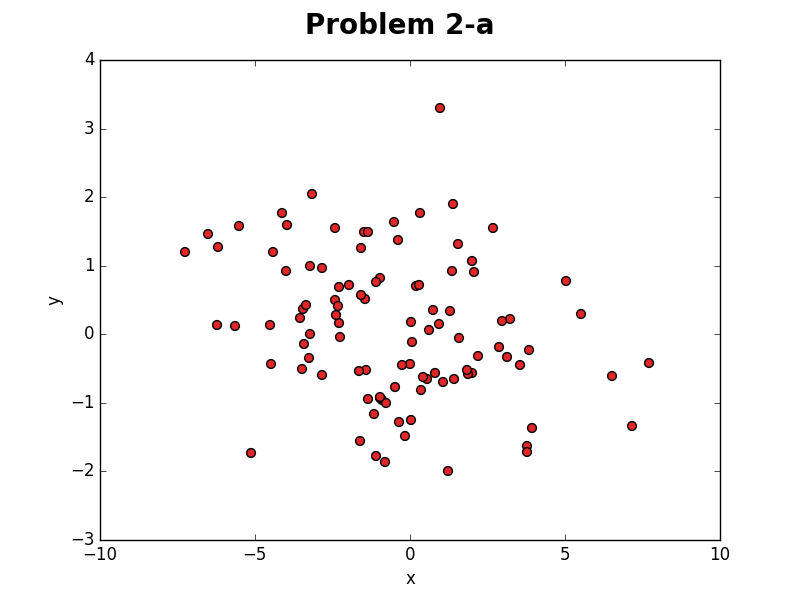
\includegraphics[width = \textwidth]{./code/2-a.png}
	}
	\label{fig:2a}
\end{figure}

\subsection*{b}
See Figure~\ref{fig:2b}
\begin{figure}[t]
	\centering{
		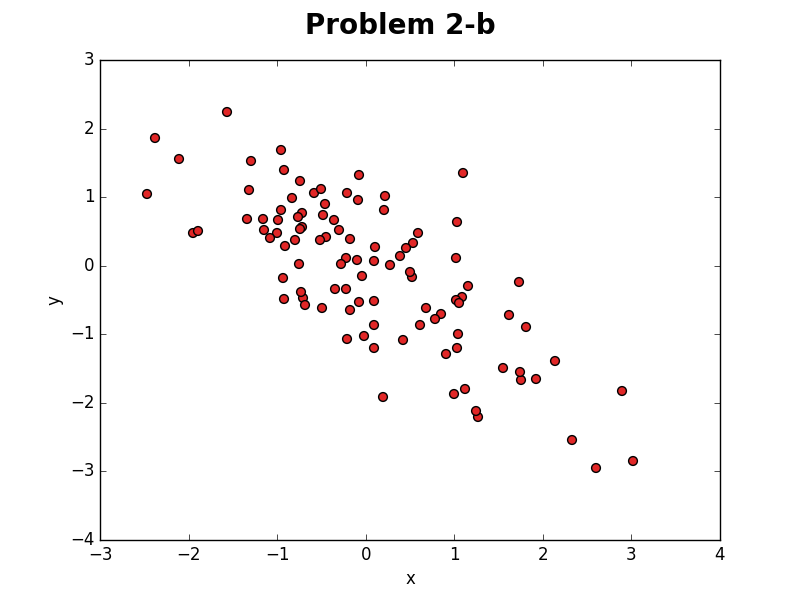
\includegraphics[width = \textwidth]{./code/2-b.png}
	}
	\label{fig:2b}
\end{figure}


\section*{Problem 3}
\subsection*{a}
See Figure~\ref{fig:3}
\begin{figure}[t]
	\centering{
		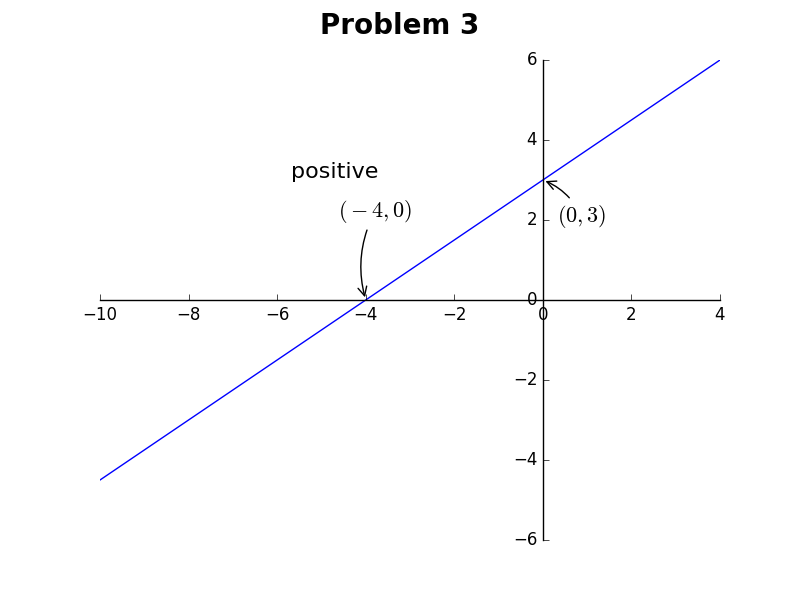
\includegraphics[width = \textwidth]{./code/3.png}
	}
	\label{fig:3}
\end{figure}

\section*{Problem 4}
\subsection*{a}
Check whether the number of distinct eigenvalues $\lambda$ is equal to $p$, and
if yes, $\sum$ is invertible, otherwise not.

\subsection*{b}
The eigenvalues of $\sum + c I$ are $(\lambda_1 + c), ... , (\lambda_p + c)$.

The eigenvectors of $\sum + c I$ are $u_1, ..., u_p$.

\subsection*{c}
The eigenvalues of $\sum^{-1}$ are $\frac{1}{\lambda_1}, ... , \frac{1}{\lambda_p} $.

The eigenvectors of $\sum^{-1}$ are $u_1, ..., u_p$.

\section*{Problem 5}
\subsection*{a}

$\mathbf{Input}$: training data $TR = (TRX_i, TRY_i)$, and testing data $T = (TX_i, TY_i)$

$\mathbf{Output}$: error rate $err$

1. For each class of digit in the training data, randomly select $20\%$ as validation data $V$, and use the remaining as training data $VTR$.

2. For each class of digit $j$ in $VTR$, calculate the $\pi_j$, which is the frequency of digit $j$. Also, calculate the mean $\mu_j$ and covariance $\sum_{j}$ of samples in class $j$.

3. Determine the label of a sample $x$ with the following equation:
\begin{align}
	\begin{split}
	\text{class}(x) &= \mathbf{max}_{j} \frac{\pi_j}{(2\pi)^{p/2} |\sum_j + c\mathbf{I}|^{0.5}}
	\text{exp}(-\frac{1}{2} (x - \mu_j)^T (\sum{}_j + c\mathbf{I})^{-1} (x - \mu_j))
	\end{split}
\end{align}.
Apply logarithm to the inner term to avoid overflow and underflow.

4. Select proper $c$ that minimize the error rate on validation dataset.

5. Use the selected $c$ to train a multivariate Gaussian on full training dataset $TR$, and calculate the error rate $err$ on the test dataset $T$.

\subsection*{b}
The error rate on the MNIST dataset is $4.17\%$.

\section*{Problem 6}
\subsection*{a}
Given a sample $x$, let
$P(Y = i | X = x)$ be the probability that $x$ belongs to class $i$. We make decision with the following equation:

\begin{equation}
\eta(x) = \left\{ \begin{array}{ll}
abastain & \mbox{if $\frac{\max \{P(Y=i | X = x ), i = 0,...9 \} }{\text{snd} \{P(Y=i | X = x ), i = 0,...9 \}}  $} \leq threshold \\
\max_i \{P(Y=i | X = x )\} & \mbox{if $\frac{\max \{P(Y=i | X = x ), i = 0,...9 \} }{\text{snd} \{P(Y=i | X = x ), i = 0,...9 \}} $} > threshold \end{array} 
\right.
\end{equation}

where $\text{snd}$ means the second largest value in an array. That is, when the ratio between largest probability and second largest probability is smaller than a ratio, the classifier abstains.


\subsection*{b}
$\mathbf{Input}$: training data $TR = (TRX_i, TRY_i)$, and testing data $T = (TX_i, TY_i)$, smoothing factor $c$, abstain fraction $f$

$\mathbf{Output}$: error rate $err$

1. For each class of digit in the training data, randomly select $20\%$ as validation data $V$, and use the remaining as training data $VTR$.

2. For each class of digit $j$ in $VTR$, calculate the $\pi_j$, which is the frequency of digit $j$. Also, calculate the mean $\mu_j$ and covariance $\sum_{j}$ of samples in class $j$.

3. Calculate the probability of the samples in $VTR$ belonging to each class,
as well as the ratio between largest probability and second largest probability.
\textbf{Set $treshold$ to the $f*100$-th percentile of the ratio}. 

4. Train a multivariate Gaussian on the whole training dataset $TR$, and evaluate the model on the test dataset with the $treshold$. Calculate the error rate $err$.

\subsection*{c}

\end{document}
